\graphicspath{{Chapitre_4/Images/}}
\chapter{Brayton cycle}\label{C4}
%%%%%%%%%%%%%%%%%%%%%%%%%%%%%%%%%%%
%%%%%                         %%%%%
%%%%% Introduction chapitre 4 %%%%%
%%%%%                         %%%%%
%%%%%%%%%%%%%%%%%%%%%%%%%%%%%%%%%%%
\quad\, In the previous chapter, the different parts constituting the Brayton cycle have been well defined. This chapter will be devoted to the description and the performance analysis of the Brayton cycle considering various configurations.

\section{Gas turbine (GT)}
%%%%%%%%%%%%%%%%%%%%%%%%%%%%%%%%%%%
%%%%%                         %%%%%
%%%%%     <<Gas turbine>>     %%%%%
%%%%%                         %%%%%
%%%%%%%%%%%%%%%%%%%%%%%%%%%%%%%%%%%
\quad\, The gas turbine (GT) is the most basic configuration of the Brayton where only four main elements are integrated within the cycle. First, there is the compressor (COMP) that will compress the ambient air. Then, the compressed air goes through the combustion chamber (CC) to increase its temperature. Finally, the exhaust gas from the combustion chamber are expanded through the turbine (TURB) to produce mechanical power. Part of this power is consumed by the compressor. The remaining is converted into electricity using an electrical generator (G). The gas cycle have been drawn on the following Figure \ref{fig:C4_BraytonGT}.

\begin{figure}[h]
\centering
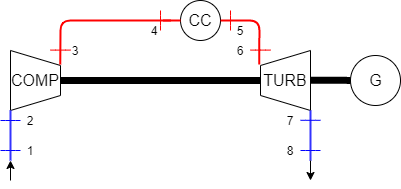
\includegraphics[width=0.5\textwidth] {GT}
\caption{Gas turbine(GT)}
\label{fig:C4_BraytonGT}
\end{figure}



As illustrated on Figure \ref{fig:C4_BraytonGT}, the cycle can be decomposed into 8 thermodynamic states. the piping between each odd and even state hasn't been illustrated for clarity. Also, it is assume that pipes only induce isotherm pressure drop.

Table \ref{tab:C4_thermo_state_GT} contains a summary of the gas cycle states emphasized on Figure \ref{fig:C4_BraytonGT}.

\begin{center}
\begin{longtable}[c]{lll}
\caption{Thermodynamic states - gas cycle (GT)}
\label{tab:C4_thermo_state_GT}\\
\hline
State n\degree & T                   & P                 \\ \hline
\endfirsthead
\multicolumn{3}{c}%
{\tablename\ \thetable\ -- \textit{Continued from previous page}} \\ \hline
State number & T                   & P                 \\ \hline
\endhead
\multicolumn{3}{r}{\textit{Continued on next page}} \\
\endfoot
\endlastfoot
State \textbf{0}: Reference state                                                            & $T_0$ = $T_{ref}$ & $p_0$ = $p_{ref}$ \\
State \textbf{1}: Ambient condition                                                          & $T_1$ = $T_{amb}$   & $p_1$ = $p_{amb}$ \\
\begin{tabular}[c]{@{}l@{}}State \textbf{2}: Inlet of the \\ compressor\end{tabular}         & $T_2=T_1$           & $p_2\leq p_1$     \\
\begin{tabular}[c]{@{}l@{}}State \textbf{3}: Outlet of the \\ compressor\end{tabular}        & $T_3>T_2$           & $p_3>p_2$         \\
\begin{tabular}[c]{@{}l@{}}State \textbf{4}: Inlet of the \\ combustion chamber\end{tabular} & $T_4=T_3$           & $p_4\leq p_3$     \\
\begin{tabular}[c]{@{}l@{}}State \textbf{5}: Outlet of the\\ combustion chamber\end{tabular} & $T_5>>T_4$          & $p_5\leq p_4$     \\
\begin{tabular}[c]{@{}l@{}}State \textbf{6}: Inlet of the\\ turbine\end{tabular}             & $T_6=T_5$           & $p_6\leq p_5$     \\
\begin{tabular}[c]{@{}l@{}}State \textbf{7}: Outlet of the \\ turbine\end{tabular}           & $T_7<T_6$           & $p_7<p_6$         \\
State \textbf{8}: Exhaust                                                                    & $T_8=T_7$           & $p_8=p_1<p_7$    
\end{longtable}
\end{center}

For each of the mentioned states, 5 thermodynamic properties are evaluated. Namely the temperature, pressure, enthalpy, entropy and density. For the last variable, the ideal gas equation (\ref{eq:C2_GP}) from the chapter \ref{C2} is used. 

A graphical representation of these states can be performed by drawing some thermodynamic diagrams. Here, the Ts and hp diagram have been drawn on Figures \ref{fig:C4_Ts_GT} and \ref{fig:C4_hp_GT}. In this chapter, all the components are supposed ideals, meaning that their corresponding efficiency are equal to 100\%.

\begin{figure}[h]
     \centering
     \begin{subfigure}[b]{0.4\textwidth}
         \centering
         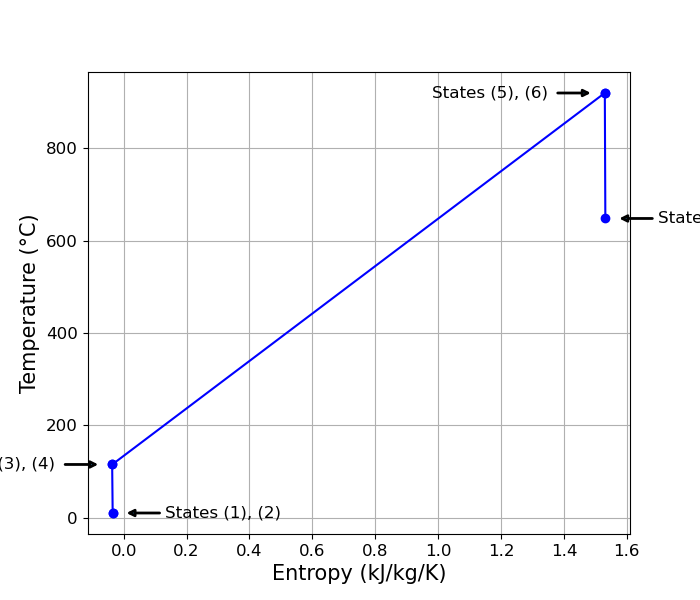
\includegraphics[width=\textwidth]{Ts_GT}
         \caption{Ts diagram - gas turbine}
         \label{fig:C4_Ts_GT}
     \end{subfigure}
     \begin{subfigure}[b]{0.4\textwidth}
         \centering
         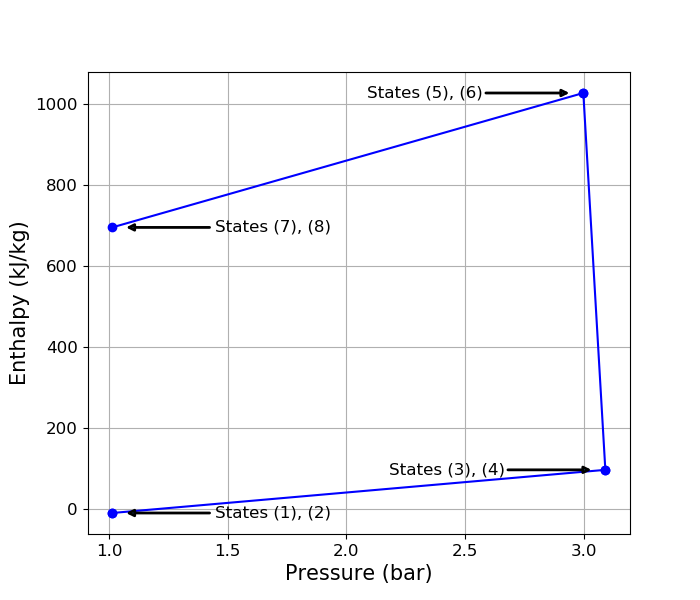
\includegraphics[width=\textwidth]{hp_GT}
         \caption{hp diagram - gas turbine}
         \label{fig:C4_hp_GT}
     \end{subfigure}
        \caption{Thermodynamic diagrams of a gas turbine}
        \label{fig:C4_thermo_diagram_GT}
\end{figure}\newpage


As it can be noticed on the two diagrams, the cycle is not closed. Indeed, the state \textbf{1} of the cycle does not correspond to to the final state. For this configuration, the exhaust gas temperature is a little bit higher than 600\degree C. Thus, there is still compared to the ambient condition 580\degree C of "thermal energy" that could be used.

The efficiency of the cycle (or thermal efficiency), based on the definition given in the chapter \ref{C2}, is equal to $\sim 24$\%. Considering the loss of energy in the exhaust gas, this efficiency can be improved.

\section{Regenerative gas turbine (RGT)}
%%%%%%%%%%%%%%%%%%%%%%%%%%%%%%%%%%%
%%%%%                         %%%%%
%%%%%    <<regenerative>>     %%%%% 
%%%%%     <<Gas turbine>>     %%%%%
%%%%%                         %%%%%
%%%%%%%%%%%%%%%%%%%%%%%%%%%%%%%%%%%
\quad\, As seen in the previous section, the gas cycle does not have a really high efficiency. However, this efficiency can be nearly tripled by adding a regenerator to the cycle. The purpose of this heat-exchanger is to transfer part of the thermal energy from the hot gas exiting the turbine to the cold flow exiting the compressor. A schematic of the regenerative gas turbine (RGT) and the associated Ts and hp diagrams are given on Figures \ref{fig:C4_RGT} and \ref{fig:C4_thermo_diagram_RGT}. 

\begin{figure}[h]
\centering
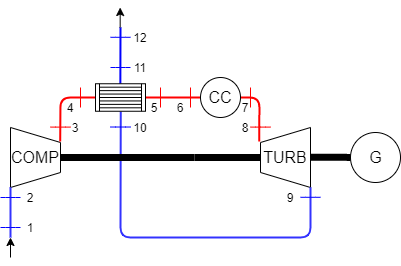
\includegraphics[width=0.5\textwidth]{RGT}
\caption{Regenerative gas turbine(RGT)}
\label{fig:C4_RGT}
\end{figure}
\begin{figure}[h]
     \centering
     \begin{subfigure}[b]{0.4\textwidth}
         \centering
         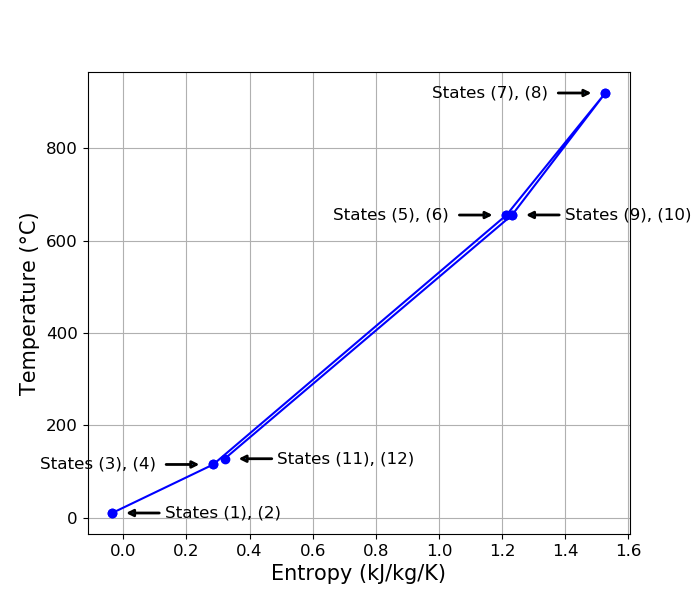
\includegraphics[width=\textwidth]{Ts_RGT}
         \caption{Ts diagram - regenerative gas turbine}
         \label{fig:C4_Ts_RGT}
     \end{subfigure}
     \begin{subfigure}[b]{0.4\textwidth}
         \centering
         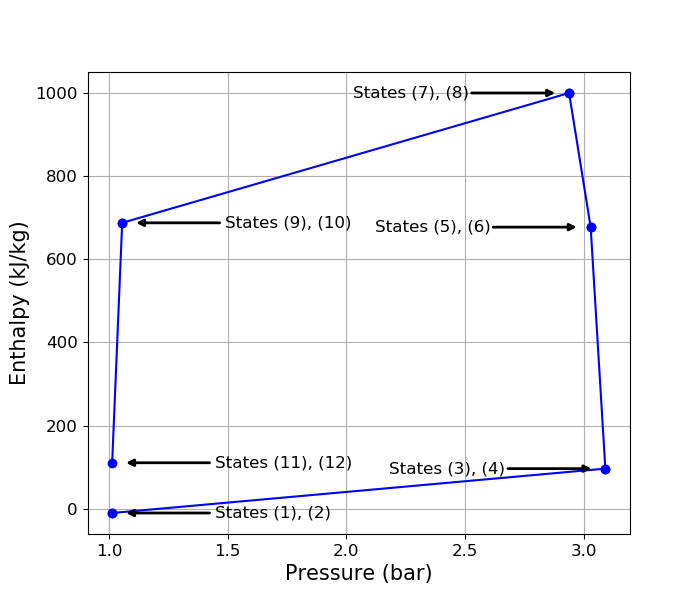
\includegraphics[width=\textwidth]{hp_RGT}
         \caption{hp diagram - regenerative gas turbine}
         \label{fig:C4_hp_RGT}
     \end{subfigure}
        \caption{Thermodynamic diagrams of a regenerative gas turbine}
        \label{fig:C4_thermo_diagram_RGT}
\end{figure}
\newpage
This has two advantages. The first one is to reduce the temperature of the gas at the exit of the cycle. The second is to reduce the fuel consumption of the system. Indeed, for an identical combustor outlet temperature (here, 950\degree C), the amount of energy that the combustion chamber has to provide to the air is lower than for the GT since the inlet temperature of the air is higher. Considering a mass flow rate of air of 180g/s, the fuel consumption goes from 3.41g/s to 1.18g/s for the RGT.

After computation, the thermal efficiency of the RGT is evaluated at $\sim$ 63\%, which is more than twice the efficiency of the GT.

Aside the regerator, a water heat exchanger (WHX) can be used to absorb the remaining from the exhaust gas to utilize it for water heating. Considering the fact that components does not have an efficiency of 100\%, the temperature at the outlet of the regenerator (state \textbf{11}) is around 200\degree C. This temperature is enough to heat up water to a target temperature of 70-80\degree C.

Even if it is beyond the scope of this master thesis, the integration of an organic rankine cycle (ORC) in place of the WHX to convert the remaining heat into electricity can also be considered\citep{Quoilin2008}.

\section{Brayton cycle - variants}
%%%%%%%%%%%%%%%%%%%%%%%%%%%%%%%%%%%
%%%%%                         %%%%%
%%%%%      <<Variants>>       %%%%%
%%%%%                         %%%%%
%%%%%%%%%%%%%%%%%%%%%%%%%%%%%%%%%%%
The GT and RGT are not the only configurations of the Brayton cycle. There exists many other involving multiple compressors, turbines, combustion chamber,etc... These configurations are illustrated in the annex \ref{annex:Brayton_variant}.

It exists many variants many variants of the Brayton cycle because engineers wanted to cover a large numbers of applications. For instance, when a large compression ratio is desired, using only one compressor is not possible. Therefore, it is necessary to split the compression between a low pressure and a high compressor. 
